\section{Navigation}
	La navigation est une science qui permet de connaitre sa position sur la Terre, calculer la route à suivre pour atteindre une autre position, ou calculer toute autre information relativement au déplacement. \\

	Les techniques de navigation utilisées dans l'aéronautique sont reprises de celles alors utilisées dans la navigation maritime (avec, aux tous débuts de l'aviation l'utilisation de sextants pour s'orienter la nuit à partir des étoiles, puis la création de phares de navigation aérienne). Ces techniques permettaient de naviguer par temps clair, mais trouvaient rapidement leurs limites pour naviguer par conditions météo médiocres ou mauvaises.
	
	\begin{center}
	\begin{minipage}[c]{1.0\linewidth}
	\begin{figure}[H]
	\begin{minipage}[c]{0.4\linewidth}
	\centering
	\includegraphics[width=0.7\linewidth]{02-Navigation/img/Phare-aéronautique-de-Baziege.jpg}
	\legende{Le phare aéronautique de Baziège (construit en 1925)}{img:Phare-aéronautique-de-Baziege}
	\end{minipage}
	\begin{minipage}[c]{0.6\linewidth}
	\centering
	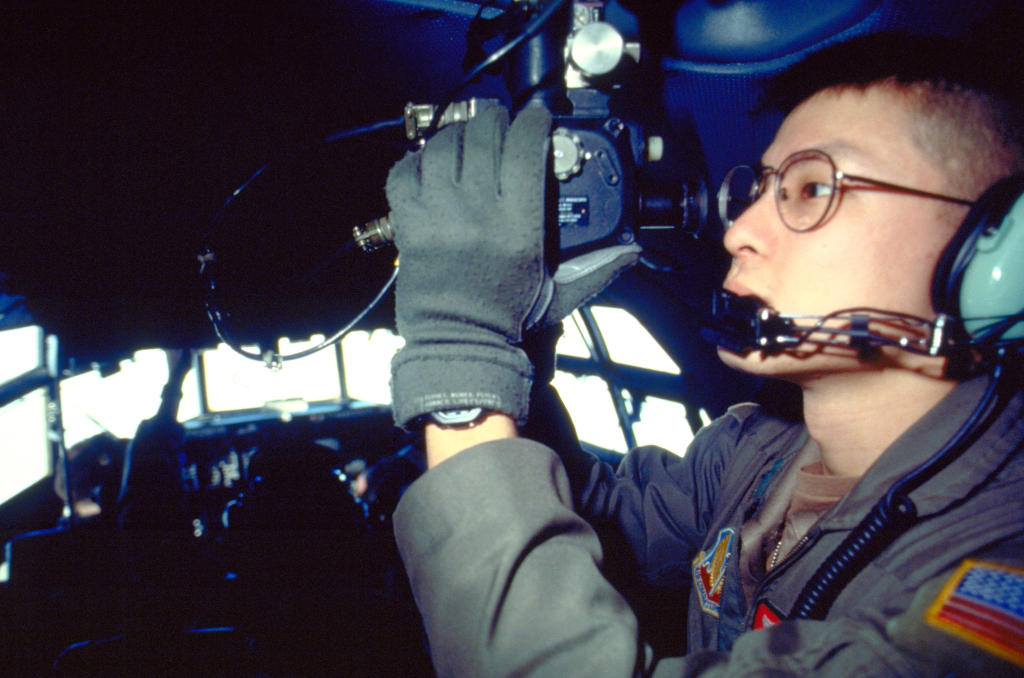
\includegraphics[width=0.95\linewidth]{02-Navigation/img/Sextant-C130.jpg}
	\legende{Utilisation d'un sextant dans un C130 (1996)}{img:Sextant-C130.jpg}
	\end{minipage}
	\end{figure}
	\end{minipage}
	\end{center}
	
	Peu à peu, les aviateurs ont donc développé des systèmes de radionavigation (NDB en 1920) qui utilisent des signaux radioélectriques plutôt que lumineux et visuels pour le repérage. Ces procédés de radionavigation fonctionnent de jour comme de nuit et sont utilisables par tous temps. Ces systèmes offrent aussi des portées bien supérieures à ceux des systèmes lumineux, ce qui permet alors d'envisager un maillage qui offre une couverture continentale. Ils nécessitent cependant des récepteurs embarqués dans les aéronefs pour être utilisables.
	
	Depuis les années 1970, la navigation aéronautique exploite de plus en plus les systèmes de navigation par satellite.\\
	
	Dans ce chapitre, nous allons étudier dans un premier temps quels sont les grands principes de la navigation aérienne, puis comment on se sert des systèmes de radionavigation.
	
	\subsection{Les grands principes de navigation}
		\subsubsection{Navigation à l'estime et cheminement à vue}
		\subsubsection{Route vraie, route magnétique, cap vrai, cap magnétique, déclinaison, déviation}
		\subsubsection{Distance entre deux points d'une carte}
		\subsubsection{Régimes de vol}
		Un aéronef évolue toujours selon des règles partagées. Pour les vols civils, on dit que l'on évolue selon les règles de la \textbf{\acrlong{cag}}	(\acrshort{cag}). La CAG défini 2 grandes régimes de vol : le VFR et l'IFR.\\
		
		Il existe d'autres règles de circulation aérienne, on peut citer par exemple la CAM (Circulation Aérienne Militaire) ou encore la CER (Circulation d'Essais et de Réception). Ces circulations ne seront pas abordées ici.
		
		\paragraph{Le vol à vue}
		Le vol \acrshort{vfr} (\anglais{\acrlong{oaci}} - règles de vol à vue) correspond historiquement au premier mode de navigation utilisé pour se déplacer en avion. Dans ce mode de navigation, on navigue principalement grâce à des repères au sol, et on pilote l'attitude de l'avion grâce a l'horizon naturel. 
		
		L'instrumentation minimale pour ce type de vol est très réduite. On peut naviguer aisément en VFR avec seulement un anémomètre (pour connaitre sa vitesse), une boussole (pour connaitre son cap) et une montre (pour mesurer le temps avant d'atteindre le prochain point de repère de la navigation), même si aujourd'hui les appareils exploités en VFR sont généralement équipés d'une instrumentation bien plus élaborée.
		
		\astuce{En français, on dit parfois VFR peut être traduit par \textbf{Voies-Ferrées/Routes} car pour naviguer selon les règles VFR on utilise des repères au sol, dont les routes et les voies ferrées.}
		
		Le principal inconvénient de ce mode de navigation est qu'il nécessite que les conditions météo soient suffisamment bonnes pour que l'horizon demeure visible et que les points de repères au sol soient identifiables. Ce régime de vol n'est donc utilisable que par beau temps. Les conditions de vols requises pour le vol VFR sont appelées \acrshort{vmc} (\anglais{\acrlong{vmc}} - conditions de vol à vue). Les conditions VMC définissent des visibilité horizontales et des distance par rapport aux nuages minimales permettant de voler à vue. Ces valeurs minimales dépendent de l'espace ou l'aéronef évolue.
		
		\info{Il est possible de voler selon les règles VFR la nuit, on parle alors de NVFR \anglais{Night VFR}.}
		
		\info{Il est possible de se servir des instruments de radionavigation ou du GPS pour naviguer en VFR, toujours en gardant les conditions VMC.}
		
		Aujourd'hui, ce mode de navigation reste très utilisée pour l'aviation de loisir mais également pour bon nombre de missions professionnelles (évacuations sanitaires, héliportage, surveillance d'infrastructures, largages de parachutistes...). \\
		
		Pour offrir des capacités de vol par conditions météo dégradées, il a donc fallu inventer un autre régime de vol : l'IFR.
		
		\paragraph{Le vol aux instruments}
		Le vol \acrshort{ifr} (\anglais{\acrlong{ifr}} - règles de vol aux instruments) définis les règles et procédure permettant de voler par tout temps, lorsque les conditions \acrshort{vmc} ne sont plus réunies. On se trouve alors en conditions \acrshort{imc}(\anglais{\acrlong{imc}} - conditions de vol aux instruments).
		
		Dans ces conditions, les informations visuelles obtenues par le sens du pilote (essentiellement la vue) ne permettent plus de piloter l'attitude de l'avion (absence d'horizon naturel) ni de naviguer (les repères au sol tout comme les obstacles sont cachés par la mauvaise visibilité, et deviennent invisibles ou visibles trop tardivement). Dans ces conditions, les pilotes vont donc se baser sur des références instrumentales pour le pilotage :
		\begin{itemize}
		\item horizon artificiel pour piloter l'attitude de l'appareil,
		\item radiobalises, guidage radar ou plus récemment GPS pour la navigation.
		\end{itemize}
		
		On constate que cette règle de navigation nécessite une instrumentation plus élaborée. Par ailleurs, il est nécessaire que l'avion et le pilote soient qualifiés pour l'IFR. Si on souhaite se poser sur un aéroport en conditions IMC, il faut également que cet aéroport soit qualifié pour l'IFR.
		
		\info{Un aéronef qui évolue selon les règles \acrshort{ifr} peut évoluer en conditions \acrshort{vmc}.}
		
		\info{Bien que la plupart des vols soient menés selon un seul régime de vol, il est cependant possible de changer de régime de vol durant le vol, sous réserve que l'avion, le pilote et éventuellement l'aéroport soient qualifiés pour l'IFR. Il est par exemple possible de réaliser le décollage et la croisière en VFR, puis de passer en IFR à l'arrivée si les conditions à l'aéroport de destination sont IMC.}
		
		\paragraph{Le VFR spécial} 
		Il existe un régime de vol particulier appelé VFR Spécial. Ce régime de vol n'est possible qu'en espace aérien contrôlé. Ce régime de vol permet d'abaisser les conditions de vol VMC en espace aérien contrôlé.
		
		\exemple{Pour évoluer dans une CTR de classe D, les conditions VMC exigent 5000~m de visibilité et de conserver 300~m d'espacement vertical et 1500~m d'espacement horizontal avec les nuages. Un pilote qui évoluerait en espace de classe D avec 4000~m de visibilité serait donc en conditions IMC. En passant en VFR spécial, les conditions météo peuvent être ramenées à 1500~m de visibilité et hors des nuages.}
		
		Le VFR spécial est soumis à \textit{clearance} du contrôle aérien. La délivrance de la \textit{clearance} impose alors au contrôleur d'assurer la séparation entre le vol VFR spécial et les vols IFR.
		
	
	\subsection{Les outils de navigation}
		\subsubsection{Cartes aéronautiques}
		
		\subsubsection{Aides à la navigation}
			\paragraph{Notions de base}
			
			\paragraph{Le VOR}
			Le \acrshort{vor} (\anglais{\acrlong{vor}}
			
			\subparagraph{Le DME}
			Le \acrshort{dme} (\anglais{\acrlong{dme}} (souvent désigné VOR-DME car traditionnellement les DME sont couplés à un VOR)
			
			\alert{De par son fonctionnement, le DME mesure une distance oblique entre le récepteur et l'émetteur. \\ Ainsi, l'équipage d'un aéronef qui passerait à la verticale d'un DME à 6000 pieds verra s'afficher 2 km et non 0.}
			
			\paragraph{L'ADF}
			L'\acrshort{adf} (\anglais{\acrlong{adf}} désigne l'équipement de réception des balises \acrshort{ndb} (\anglais{\acrlong{ndb}}.
			
			\paragraph{Le goniomètre}
			Le \gls{goniomètre}
			
			\paragraph{Le GPS}